%====================================================================================================
\chapter{Evaluation of the Emulator for L0 Muon Trigger System} \label{ch:L0MuonEmulator}
%====================================================================================================
This chapter introducts the evaluation of the emulator emulating the L0 muon trigger behavior on both barrel and endcap region, which will be called as L0MuonEmulator in this paper. The L0MuonEmulator is an existing C++ based software package on Athena that emulates the trigger decision for muons as a part of L0 trigger system for HL-LHC. The L0MuonEmulator make decisions of whether a muon candidate should be accepted or rejected based on a filtering model with pre-set parameters of posibility and a "smearing" algorithm that imitate the detector response due to the position resolution of the detectors. In this chapter, we first provide an overview of the emulator's design and logic. Next, we discuss the limitations of current muon trigger geometric due to muon detectors structure, and then made a praticle approach on the emulator to incorporate the limitations. Finally, we evaluate the performance of the emulator and highlight the need for a more precise simulation approach.
%====================================================================================================
\section{Overview} \label{sec:L0MuonEmulatorOverview}
%====================================================================================================
The purpose of the L0MuonEmulator is to provide a fast emulation of the Level-0 muon trigger response, using generator-level truth muons as input. At present, the emulator takes as input the \texttt{xAOD::TruthParticleContainer} containing all generated particles in a simulated Monte Carlo event and selects only final-state muons (with PDG ID $\pm13$ and status 1) that satisfy basic kinematic criteria of $p_\mathrm{T} > 2$~GeV. These selected muons are then passed through a smearing and filtering procedure that models the detector resolution and trigger efficiency, and the final output is a collection of emulated L0 muon Region-of-Interest (RoI) objects, stored in an data container \texttt{xAOD::MuonRoIContainer}. Each RoI includes information such as transverse momentum ($p_\mathrm{T}$), pseudorapidity ($\eta$), azimuthal angle ($\phi$), and charge.

The filtering model in the L0MuonEmulator is designed to simulate the trigger efficiency as a function of muon transverse momentum. A simplified step-function model is implemented, in which muons below a certain threshold (currently 3~GeV) are discarded with 100\% inefficiency, while muons above that threshold are accepted with a fixed efficiency of 95\%. In addition, the emulator includes a basic geometric masking procedure to exclude regions outside the muon detector acceptance. Currently, this is implemented by discarding all truth muons with pseudorapidity $|\eta| > 2.41$, which roughly corresponds to the coverage limit of the L0 muon trigger chambers in ATLAS. Truth muons outside this region are automatically rejected.

The smearing algorithm emulates the detector resolution by applying a Gaussian fluctuation to the inverse transverse momentum ($q/p_\mathrm{T}$) of the selected muons. The width of the Gaussian (i.e., the resolution) is parameterized as 5\% of the input $q/p_\mathrm{T}$ value. The $\eta$ and $\phi$ positions are not smeared at this stage, as the resolution of the RoI granularity is coarser than the smearing scale, and the binning dominates the uncertainty. Once smeared, the kinematic variables are encoded into a bit-wise RoI word format compatible with the hardware-level representation used in the ATLAS trigger system.

Currently, the L0MuonEmulator provides several functionalities beyond simple emulation. It includes an extensive monitoring infrastructure based on the Athena Monitoring Framework. A series of histograms are automatically produced during the execution to validate the emulator output against the input truth muon properties. These include distributions of $\eta$, $\phi$, $p_\mathrm{T}$, and $q/p_\mathrm{T}$ before and after smearing, as well as resolution plots such as $\Delta\eta$, $\Delta\phi$, and relative $p_\mathrm{T}$ deviation. These features support the evaluation of trigger-level muon reconstruction quality.

Below is a summary table of the output histograms and their corresponding physical meaning.
\begin{table}[htbp]
  \centering
  \caption{Summary of L0MuonEmulator output histograms}
  \label{tab:L0MuonPlots}
  \begin{tabular}{ll}
    \hline
    Histogram Name & Physical Meaning \\
    \hline
    track\_input\_eta     & Truth muon pseudorapidity ($\eta$) \\
    track\_input\_phi     & Truth muon azimuthal angle ($\phi$) \\
    track\_input\_pt      & Truth muon transverse momentum ($p_T$) \\
    track\_input\_curv    & Truth muon curvature ($q/p_T$) \\
    track\_output\_eta    & Smeared muon pseudorapidity \\
    track\_output\_phi    & Smeared muon azimuthal angle \\
    track\_output\_pt     & Smeared muon transverse momentum \\
    track\_output\_curv   & Smeared muon curvature ($q/p_T$) \\
    roi\_output\_eta      & Reconstructed pseudorapidity ($\eta$) in RoI  \\
    roi\_output\_phi      & Reconstructed azimuthal angle ($\phi$) in RoI  \\
    roi\_output\_pt       & Reconstructed transverse momentum ($p_T$) in RoI \\
    roi\_output\_curv     & Reconstructed curvature ($q/p_T$) in RoI\\
    delta\_eta            & Difference of $\eta$ between RoI and truth \\
    delta\_phi            & Difference of $\phi$ between RoI and truth\\
    delta\_pt             & Relative $p_T$ difference between RoI and truth \\
    delta\_curv           & Relative $q/p_T$ difference between RoI and truth \\
    \hline
  \end{tabular}
\end{table}

%====================================================================================================
\section{Muon Trigger Acceptence at Phase-II Upgrade} \label{subsec:MuonTriggerAcceptance}
%====================================================================================================
In the ATLAS detector, the outermost muon detection system exhibits non-uniform spatial coverage, especially in the barrel region, due to mechanical structures that support the large barrel toroid coils for magnetic system. These mechanical supports physically block the installation of detector elements, resulting in unavoidable dead zones or ``holes'' in the detector acceptance. Figure~\ref{fig:ATLAS_muon_geometry} shows a schematic overview of the ATLAS subdetectors, including the toroid coil support structures and the muon detectors, which are affected by the presence of the former.

\begin{figure}[htbp]
  \centering
  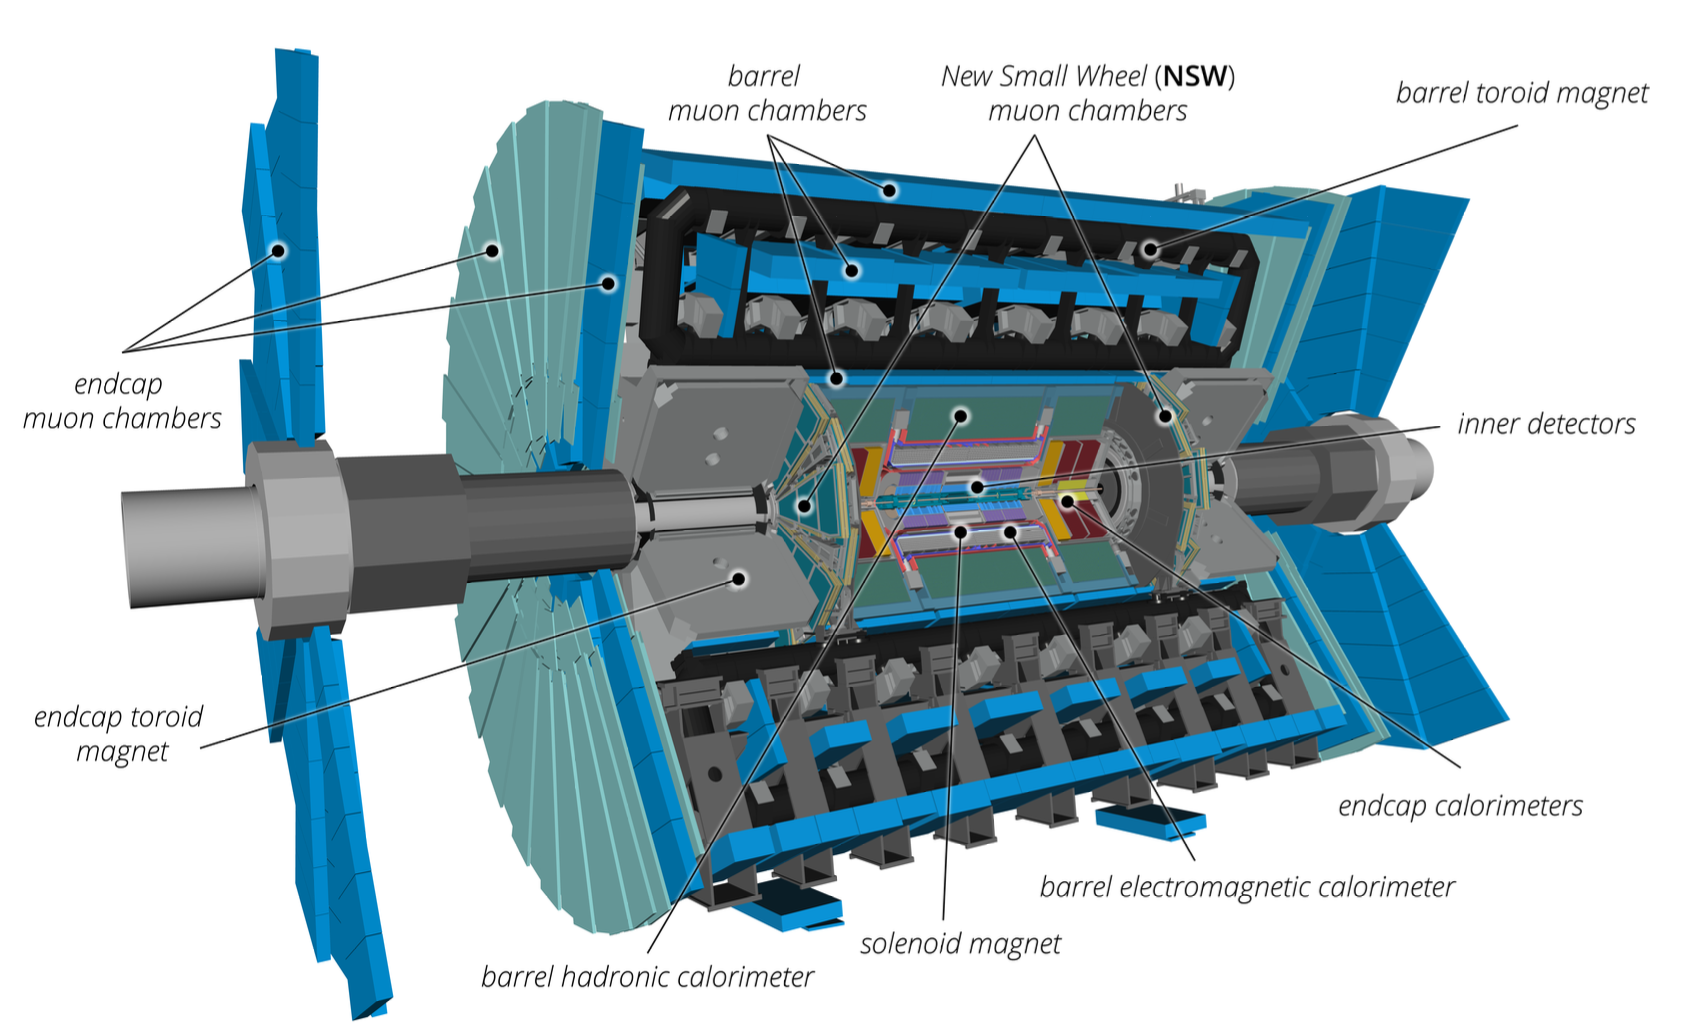
\includegraphics[width=0.8\textwidth]{figs/chapter4/ATLAS_muon_detectors_and_toroids3.png}
  \caption{Schematic layout of the ATLAS muon detector system. The support structures of the toroids introduce unavoidable coverage holes in the barrel and endcao regions \cite{ATLASRun3Detector}.}
  \label{fig:ATLAS_muon_geometry}
\end{figure}

The most affected subsystem is the Resistive Plate Chamber (\RPC) system in the barrel region. As illustrated in Figure~\ref{fig:RPC_structure}, the RPC detector has three layers currently in Run~3: two in the Barrel Middle (BM) station and one in the Barrel Outer (BO) station. Trigger decisions are based on spatial coincidences between these layers. However, the BM station suffers from blind zones caused by the presence of toroid coil supports, reducing the efficiency in affected regions.

\begin{figure}[htbp]
  \centering
  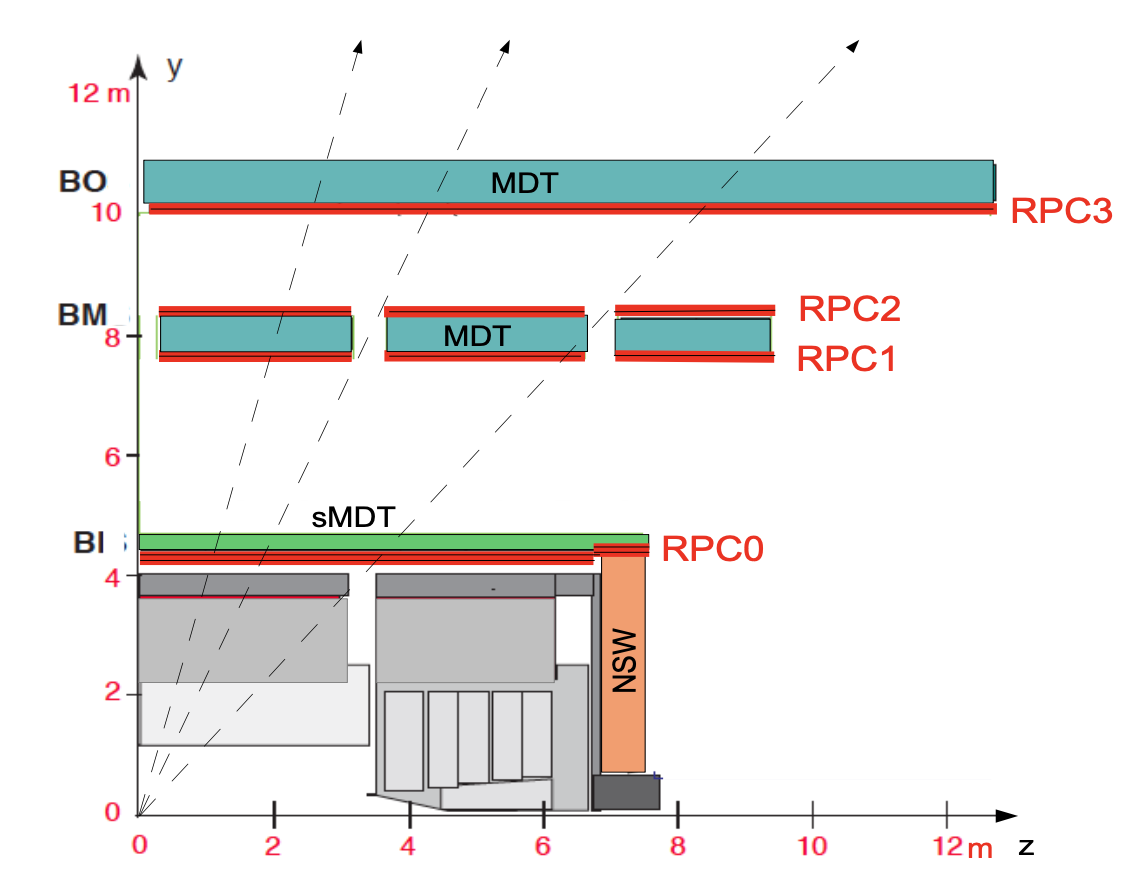
\includegraphics[width=0.7\textwidth]{figs/chapter4/RPC_detector_structure.png}
  \caption{RPC detector layout in the Run~3 barrel configuration. The two BM layers and one BO layer form the basis for L0 muon trigger coincidence logic.}
  \label{fig:RPC_structure}
\end{figure}

To overcome this limitation, the Phase-II upgrade adds a new RPC layer in the Barrel Inner (BI) station, known as RPC0. The BI region, unaffected by mechanical obstructions, offers near-complete angular coverage. This additional layer enables a four-layer RPC configuration and allows for more flexible coincidence schemes. Three main schemes are considered: “3/3 chambers”, “3/4 chambers”, and “3/4 chambers + BI-BO”. These are defined by the number of layers required to register hits in various parts of the barrel detector. A summary of the logic combinations is provided in Table~\ref{tab:RPC_coincidence_modes}.

\begin{table}[htbp]
  \centering
  \caption{Hit requirements for different RPC trigger coincidence modes.}
  \label{tab:RPC_coincidence_modes}
  \begin{tabular}{lccc}
    \hline
    Requirement & RPC0 (BI) & BM (RPC1+2) & RPC3 (BO) \\
    \hline
    3/3 chambers          & --         & 3 out of 4 & 1 out of 2 \\
    \hline
    3/4 chambers          & --         & 3 out of 4 & 1 out of 2 \\
                          & 2 out of 3 & \multicolumn{2}{c}{3 out of 6} \\
    \hline
    3/4 chambers + BI-BO  & --         & 3 out of 4 & 1 out of 2 \\
                          & 2 out of 3 & \multicolumn{2}{c}{3 out of 6} \\
                          & 2 out of 3 & --         & 1 out of 2 \\
    \hline
  \end{tabular}
\end{table}

\begin{figure}[htbp]
  \centering
  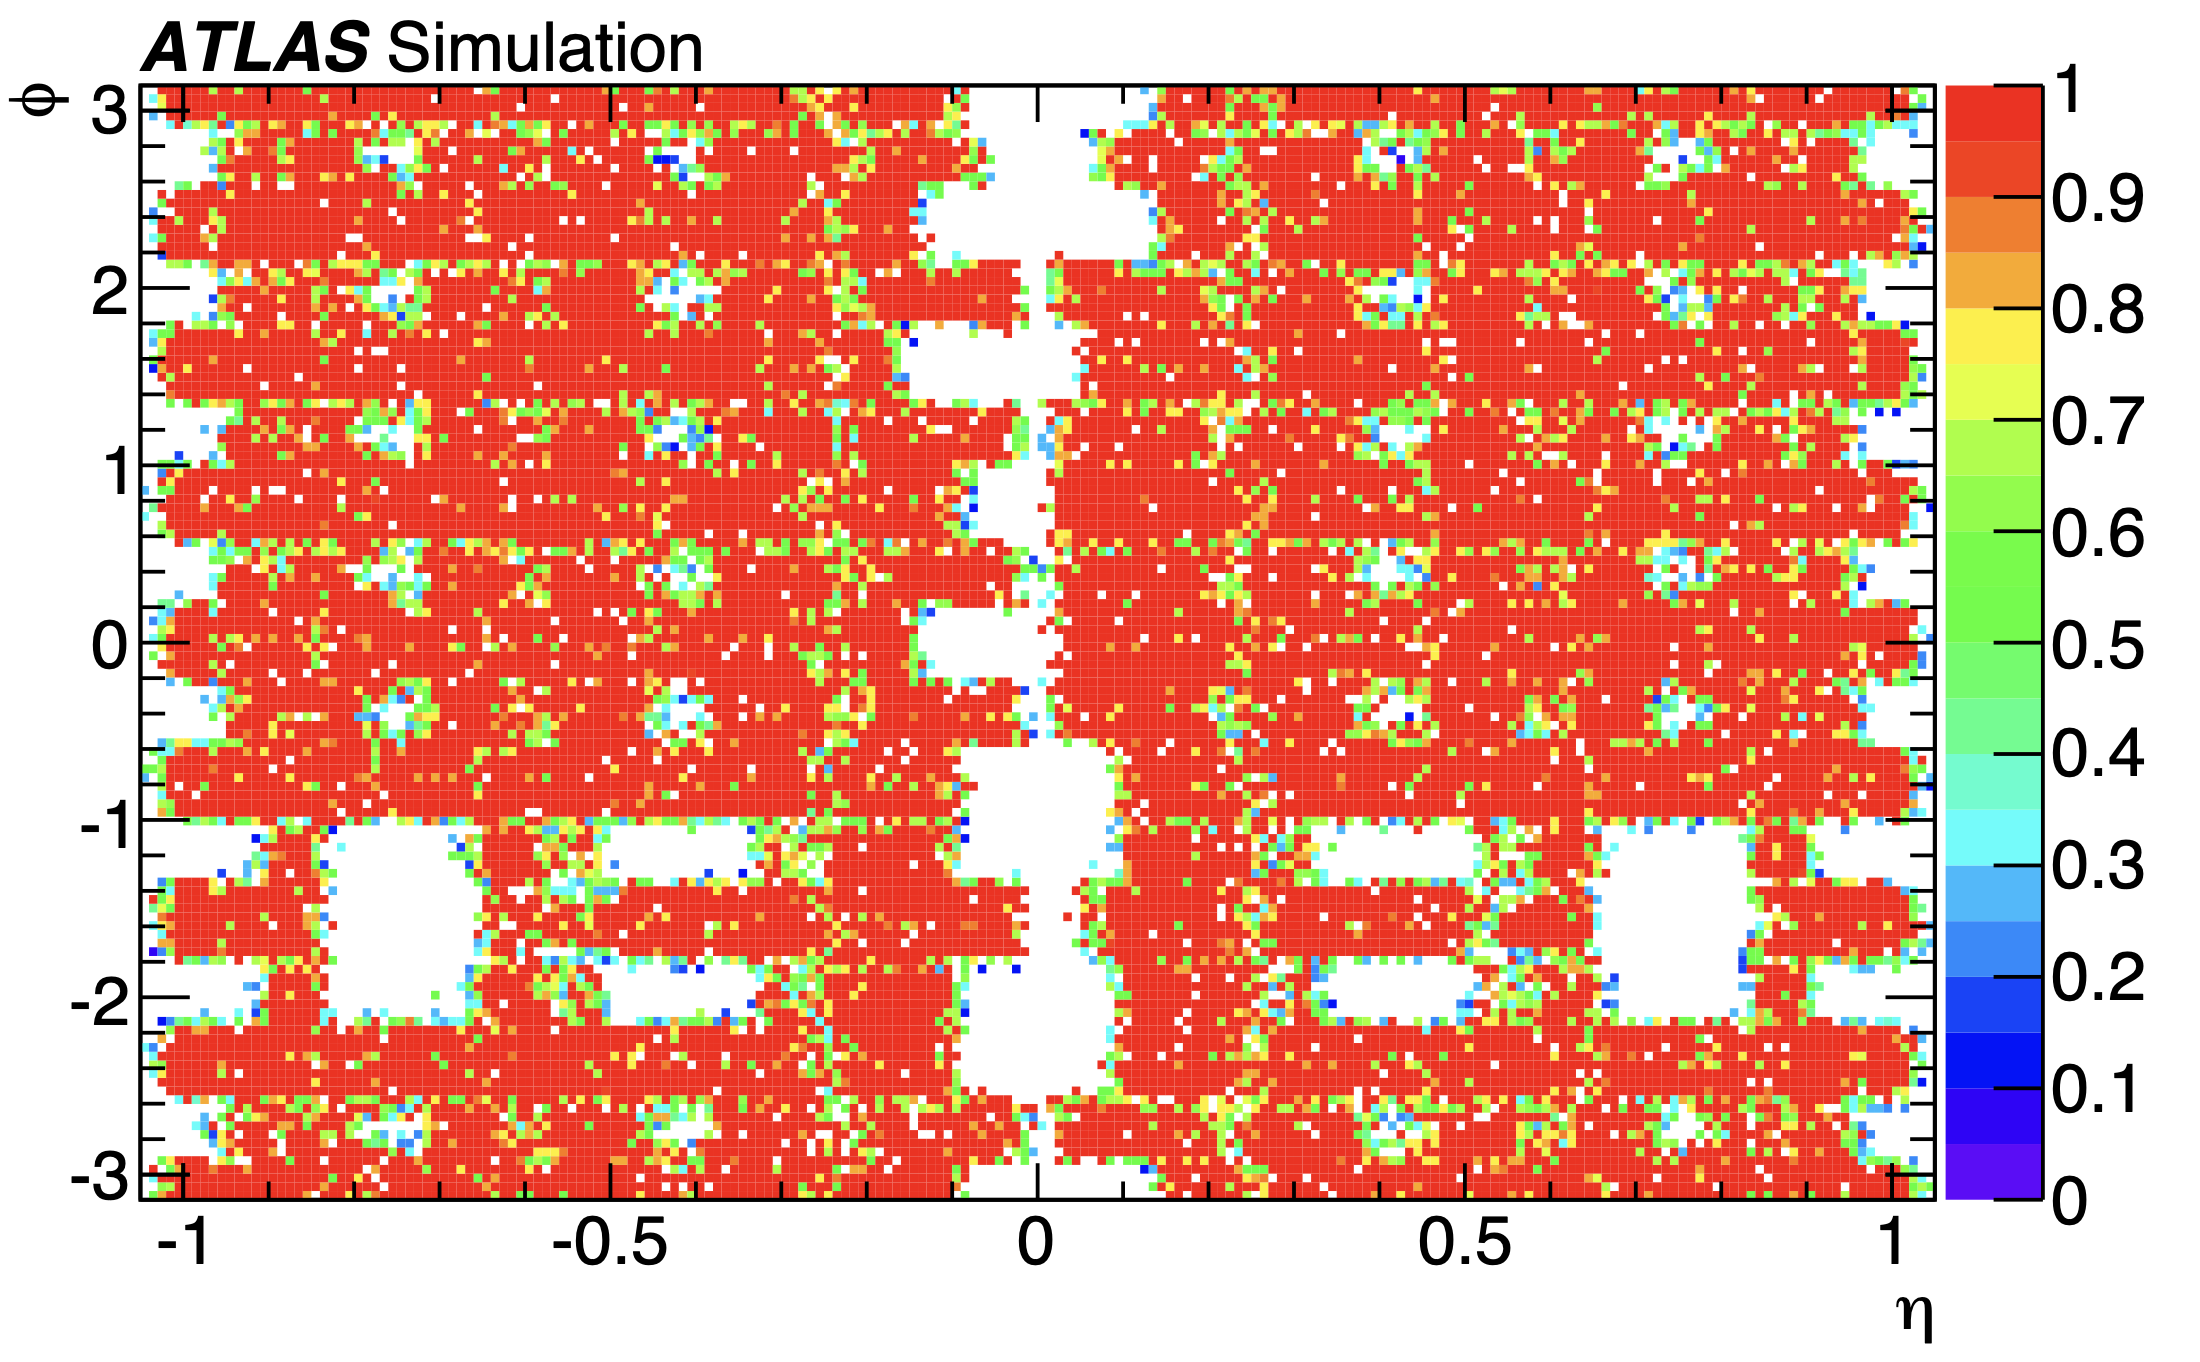
\includegraphics[width=0.75\textwidth]{figs/chapter4/trigger_acceptance_map_3_3.png}
  \caption{Trigger acceptance map in $\eta$-$\phi$ space using the 3/3 chambers coincidence logic. Significant coverage holes are visible in the BM station due to toroid coil supports.}
  \label{fig:trigger_acceptance_3_3}
\end{figure}

\begin{figure}[htbp]
  \centering
  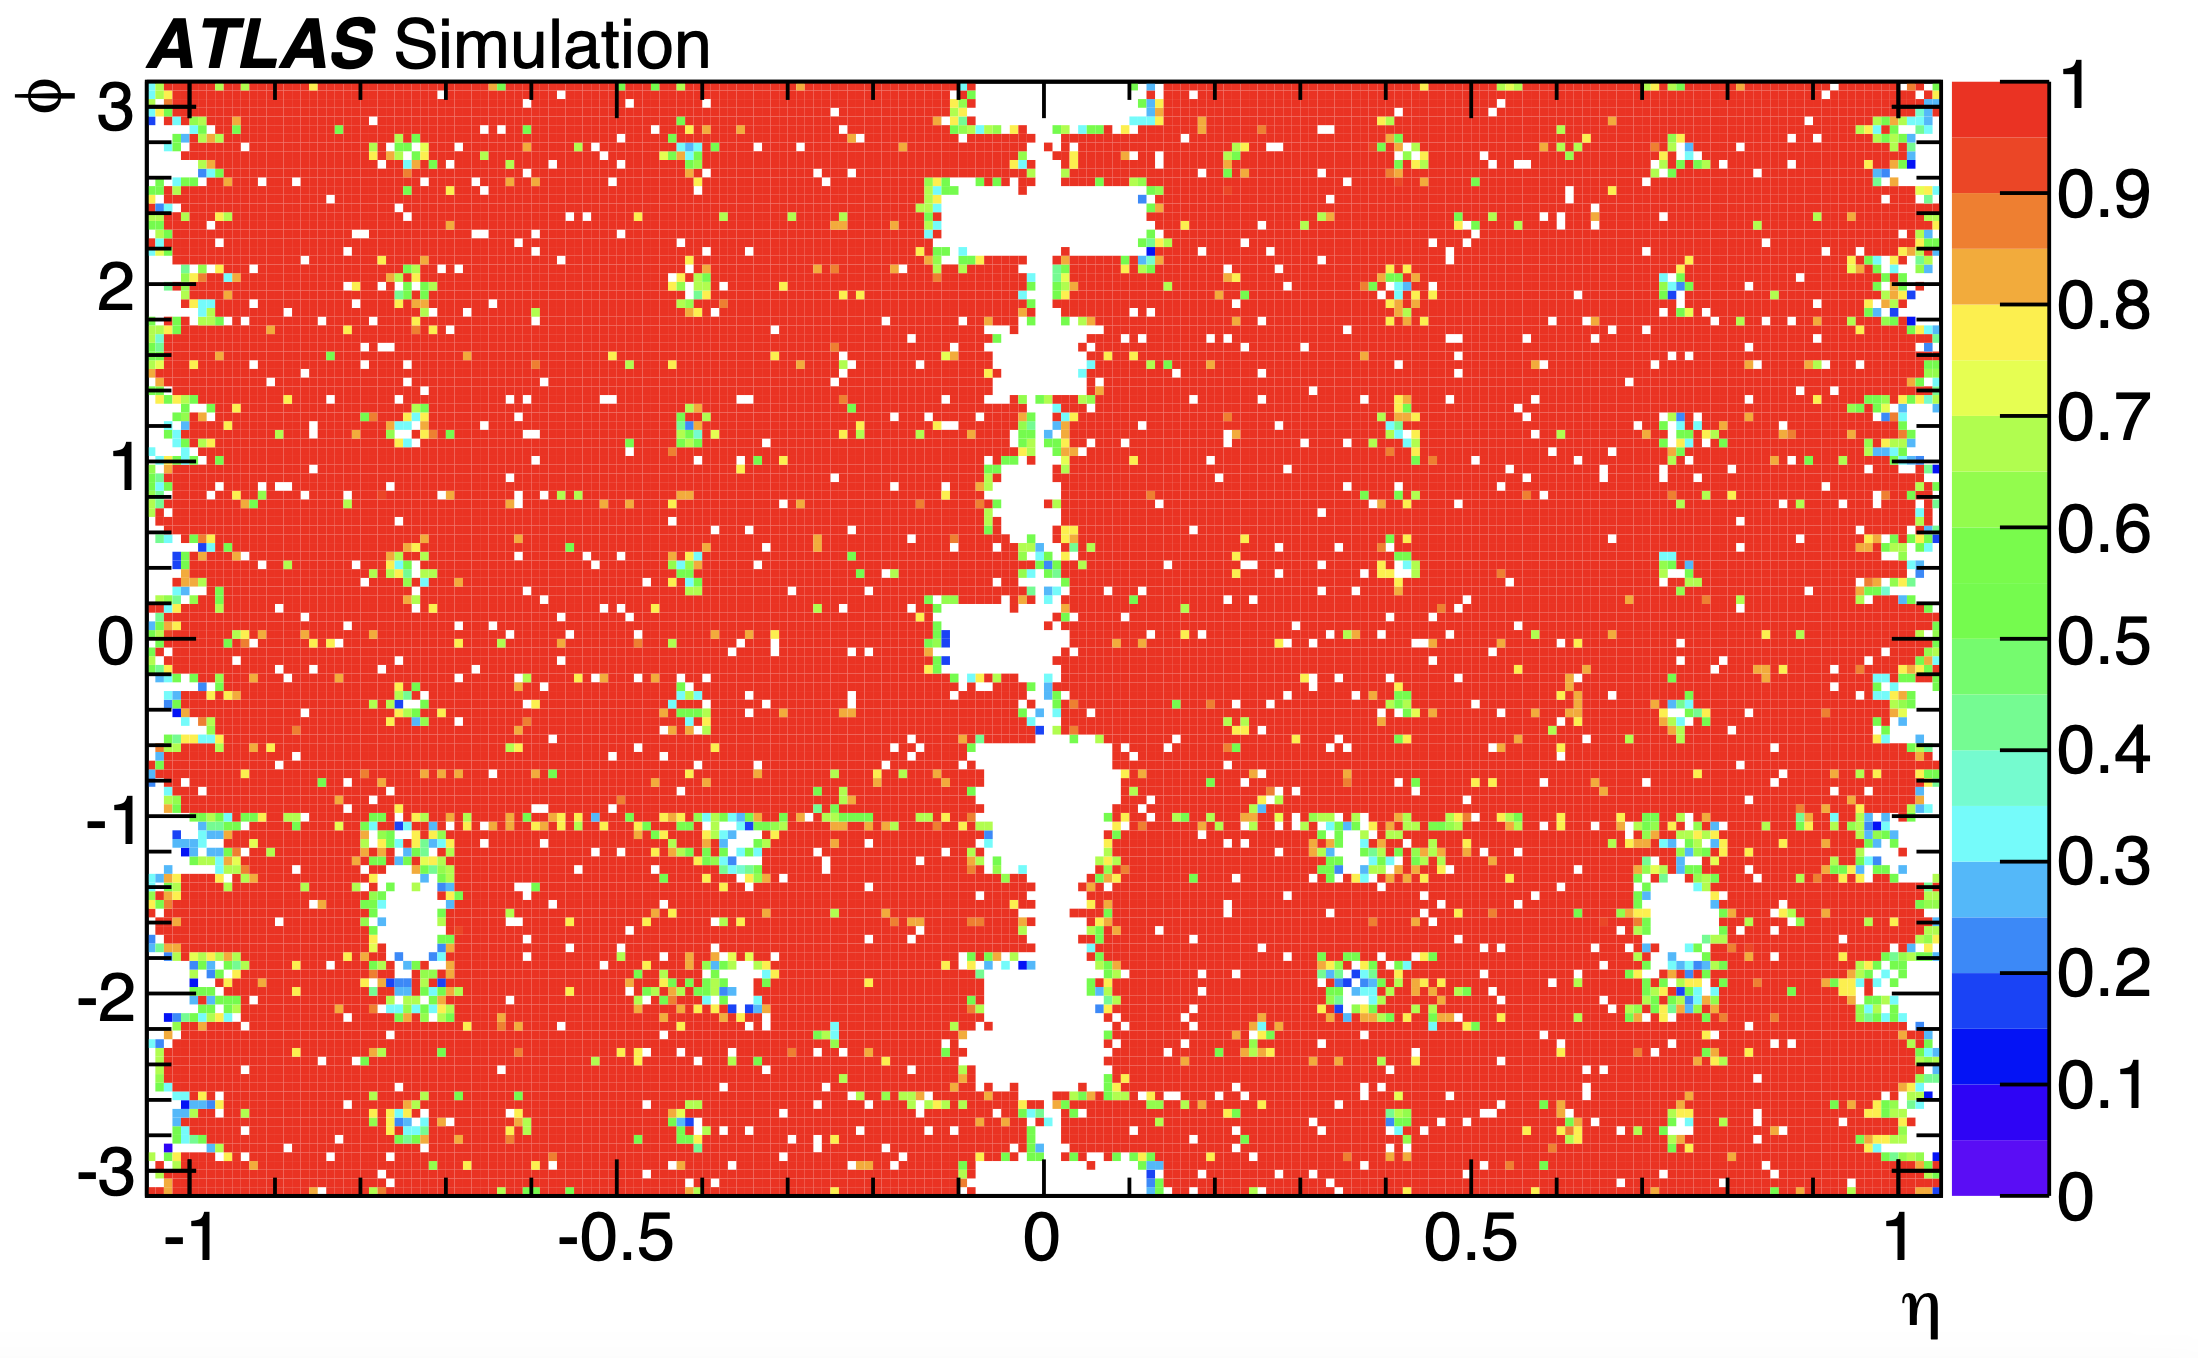
\includegraphics[width=0.75\textwidth]{figs/chapter4/trigger_acceptance_map_3_4.png}
  \caption{Trigger acceptance map with 3/4 chambers coincidence scheme. The additional RPC0 layer in the BI station significantly improves acceptance in the central barrel region.}
  \label{fig:trigger_acceptance_3_4}
\end{figure}

\begin{figure}[htbp]
  \centering
  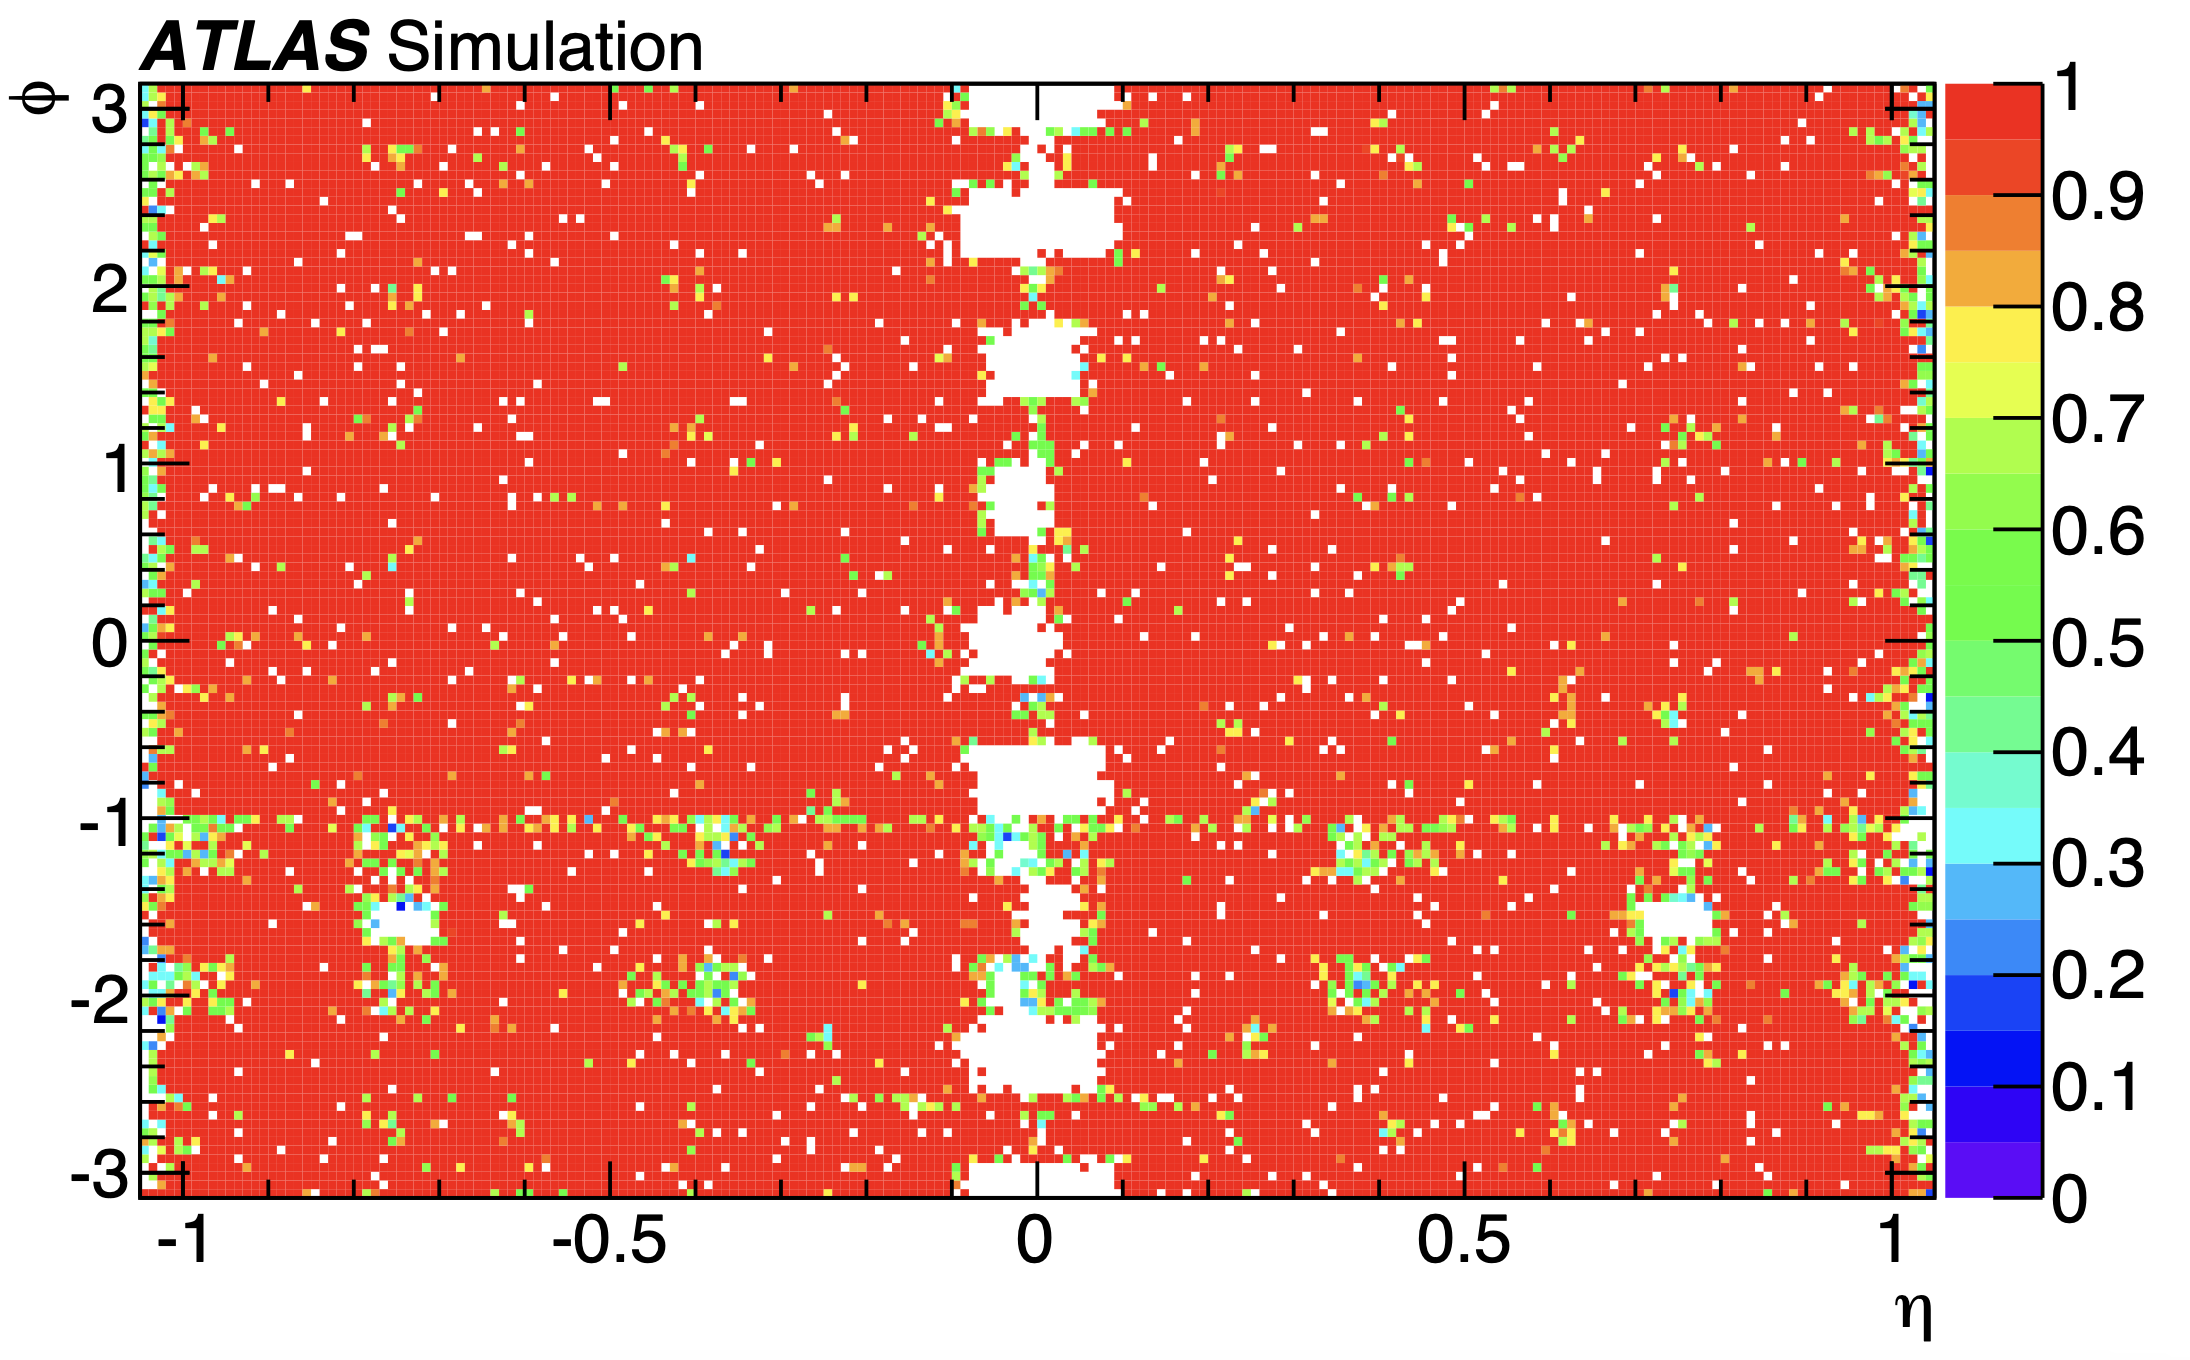
\includegraphics[width=0.75\textwidth]{figs/chapter4/trigger_acceptance_map_3_4_BI_BO.png}
  \caption{Trigger acceptance using 3/4 chambers + BI-BO logic. BI-BO mode offers further coverage in outer barrel regions.}
  \label{fig:trigger_acceptance_3_4_BI_BO}
\end{figure}

As evident from the comparison, the Phase-II RPC layout significantly enhances the trigger acceptance, particularly in the central barrel region ($|\eta| < 1.0$), by reducing most of the structural gaps through the addition of the BI station. However, even with the most inclusive coincidence mode (the 3/4 chambers + BI-BO scheme), some coverage holes remain unavoidable due to persistent mechanical limitations. In this chapter, the practical approach adopted for the emulator is based on the acceptance pattern corresponding to the 3/4 chambers + BI-BO logic, as illustrated in Figure~\ref{fig:trigger_acceptance_3_4_BI_BO}.
%====================================================================================================
\section{Practical Approach} \label{sec:RealismApproach}
%====================================================================================================
To improve the realism of the emulator, a geometry-based optimization was implemented in the smearing algorithm to account for the position dependence of the trigger efficiency in the $(\eta, \phi)$ plane.

As described in Section~\ref{sec:L0MuonEmulatorOverview}, the original implementation adopted a simplified geometric acceptance cut by discarding all truth muons with pseudorapidity $|\eta| > 2.41$, roughly corresponding to the nominal detector coverage of the L0 muon chambers. However, this approach did not account for local inefficiencies within the nominal acceptance region caused by mechanical structures such as the toroid coil supports.

To address this, we improved the emulator's practical performance by incorporating $(\eta, \phi)$-dependent masking based on the trigger acceptance map: Figure~\ref{fig:trigger_acceptance_3_4_BI_BO} discussed in Section~\ref{subsec:MuonTriggerAcceptance}. In the improved implementation, specific $(\eta, \phi)$ intervals corresponding to uncovered regions are manually vetoed within the smearing algorithm. This allows the emulator to more accurately reflect the spatial acceptance of the real detector, particularly in the barrel region where such gaps are most significant.


%====================================================================================================
\section{Performance Evaluation} \label{sec:L0MuonEmulatorPerformance}
%====================================================================================================
In this section, we evaluate the performance of the L0MuonEmulator after incorporating the geometry-based practical approach. The assessment focuses on key observables relevant to trigger behavior, including the distributions of muon transverse momentum ($p_\mathrm{T}$), pseudorapidity ($\eta$), and azimuthal angle ($\phi$) before and after trigger filtering. Additionally, the trigger efficiency as a function of $p_\mathrm{T}$ is examined to illustrate the momentum-dependent response of the emulator. Two-dimensional $(\eta, \phi)$ acceptance maps are also presented to visualize the spatial dependence of the trigger response and to facilitate a direct comparison with Figure~\ref{fig:trigger_acceptance_3_4_BI_BO}. These studies are intended to validate the emulator's consistency with the
realistic detector geometry and expected performance.

We begin with the transverse momentum ($p_\mathrm{T}$) distributions shown in Figure~\ref{fig:comparison_hist_pt}. The panel presents the $p_\mathrm{T}$ spectra before and after trigger filtering. As expected, muons with $p_\mathrm{T} < 3$~GeV are completely suppressed, while the acceptance increases gradually with $p_\mathrm{T}$. This reflects the effect of the emulator’s threshold-based filtering logic. And to evaluate the efficiency performance seperatedly in both endcap($|\eta| < 1.05$) and barred($1.05 < |\eta| < 2.41$) region, Figure~\ref{fig:eff_pt_endcap} and Figure~\ref{fig:eff_pt_barrel} gives the efficiency of $p_\mathrm{T}$ in both regions.

\begin{figure}[htbp]
  \centering
  \includegraphics[width=0.8\textwidth]{figs/chapter4/comparison_hist_pt.pdf}
  \caption{$p_\mathrm{T}$ distributions of truth muons before and after trigger filtering.}
  \label{fig:comparison_hist_pt}
\end{figure}

\begin{figure}[htbp]
  \centering
  \includegraphics[width=0.8\textwidth]{figs/chapter4/efficiency_vs_pt_endcap.pdf}
  \caption{Trigger efficiency as the function of $p_\mathrm{T}$ in endcap region.}
  \label{fig:eff_pt_endcap}
\end{figure}

\begin{figure}[htbp]
  \centering
  \includegraphics[width=0.8\textwidth]{figs/chapter4/efficiency_vs_pt_barrel.pdf}
  \caption{Trigger efficiency as the function of $p_\mathrm{T}$ in barrel region.}
  \label{fig:eff_pt_barrel}
\end{figure}

Figure~\ref{fig:comparison_hist_eta} and Figure~\ref{fig:comparison_hist_phi} show the pseudorapidity ($\eta$) and azimuthal angle ($\phi$) distributions before and after filtering. In the $\eta$ distribution, muons with $|\eta| > 2.41$ are not accepted, reflecting the emulator's geometric acceptance. Additionally, a visible dip near $\eta = 0$ appears due to the manually masked hole region. The $\phi$ distribution exhibits more uniformly distributed inefficiencies, which aligns with the emulator's $(\eta, \phi)$ veto logic.

\begin{figure}[htbp]
  \centering
  \includegraphics[width=0.8\textwidth]{figs/chapter4/comparison_hist_eta.pdf}
  \caption{Comparison of $\eta$ distributions before and after the trigger filtering.}
  \label{fig:comparison_hist_eta}
\end{figure}

\begin{figure}[htbp]
  \centering
  \includegraphics[width=0.8\textwidth]{figs/chapter4/comparison_hist_phi.pdf}
  \caption{Comparison of $\phi$ distributions before and after the trigger filtering.}
  \label{fig:comparison_hist_phi}
\end{figure}

To evaluate the emulator's spatial denpendence, Figure~\ref{fig:eta_phi_comparison} compares the two-dimensional $(\eta, \phi)$ acceptance maps: the reference map from Phase-II trigger studies (top) and the emulator-generated efficiency map (bottom). Dashed blue boxes in the right panel indicate the manually masked regions. Only obvious region around $\eta = 0$ and $|\eta| = 0.7$ are masked here, while other unobvious region are ignored here. This comparison indicates significant mismatch of both coverage and accuracy.

\begin{figure}[htbp]
  \centering
  \includegraphics[width=0.8\textwidth]{figs/chapter4/Trigger_acceptance_map_3_4_BI_BO.pdf}
  \vspace{0.5em}
  
  \includegraphics[width=0.95\textwidth]{figs/chapter4/efficiency_eta_phi_2D.pdf}
  
  \caption{Comparison of trigger acceptance maps in the $(\eta, \phi)$ plane. Top: Reference acceptance from Phase-II studies. Bottom: Emulator efficiency map with manually masked regions.}
  \label{fig:eta_phi_comparison}
\end{figure}

In conclusion, according to the efficiency performance on both $p_\mathrm{T}$ and $(\eta, \phi)$ plane, although the implemented region masking improves the realism of the emulator, it remains insufficient to meet the precision required for accurate muon trigger simulation for physics analysis. A complete simulator of high precision that simulates the trigger logic in full detail using hardware-level bitmap inputs is necessary. This motivates the development of a bitwise simulation framework based on the TGC trigger system, which will be introduced in the next chapter.
